\documentclass[times]{itmo-student-thesis}

%% Опции пакета:
%% - specification - если есть, генерируется задание, иначе не генерируется
%% - annotation - если есть, генерируется аннотация, иначе не генерируется
%% - times - делает все шрифтом Times New Roman, собирается с помощью xelatex
%% - languages={...} - устанавливает перечень используемых языков. По умолчанию это {english,russian}.
%%                     Последний из языков определяет текст основного документа.

%% Делает запятую в формулах более интеллектуальной, например:
%% $1,5x$ будет читаться как полтора икса, а не один запятая пять иксов.
%% Однако если написать $1, 5x$, то все будет как прежде.
\usepackage{icomma}

%% Один из пакетов, позволяющий делать таблицы на всю ширину текста.
\usepackage{tabularx}
\usepackage{forest}

%% Данные пакеты необязательны к использованию в бакалаврских/магистерских
%% Они нужны для иллюстративных целей
%% Начало
%\usepackage{tikz}
%\usetikzlibrary{arrows}
\usepackage{filecontents}
\begin{filecontents*}[overwrite]{bachelor-thesis.bib}
	@online{sourcecode,
		author = {Gradoboev Denis},
		title = {Исхоный код проекта},
		url = {https://github.com/DendyGrobovshik/bachelor-thesis},
		langid = {english}
	}
	
	@online{zig,
		author = {Zig Software Foundation},
		title = {Официальная документация языка программирования zig},
		url = {https://web.archive.org/web/20240511162736/https://ziglang.org/documentation/0.12.0/},
		langid = {english}
	}
	
	@online{ziggenerics,
		author = {Karl Seguin},
		title = {Generics in zig},
		url = {https://web.archive.org/web/20240309115114/https://www.openmymind.net/learning_zig/generics/},
		langid = {english}
	}
	
	@online{memorywall,
		author = {Bartłomiej Llimczak},
		title = {Memory-wall problem},
		url = {https://web.archive.org/web/20231002090943/https://developer20.com/memory-wall-problem/},
		langid = {english}
	}
	
	@online{hoogle,
		author = {Neil Mitchell},
		title = {Главная страница Hoogle},
		url = {https://web.archive.org/web/20240509155056/https://hoogle.haskell.org/},
		langid = {english}
	}
	
	@online{hooglereview,
		author = {Neil Mitchell},
		title = {Обзор Hoogle 5},
		url = {https://web.archive.org/web/20240203212114/https://neilmitchell.blogspot.com/2020/06/hoogle-searching-overview.html},
		langid = {english}
	}
	
	@online{clean,
		author = {Software Technology Research Group of Radboud University Nijmegen},
		title = {Clean wiki},
		url = {https://web.archive.org/web/20240512102324/https://wiki.clean.cs.ru.nl/Clean},
		langid = {english}
	}
	
	@online{cloogle,
		author = {Camil Staps},
		title = {Главная страница Cloogle},
		url = {https://web.archive.org/web/20240427163013/https://www.cloogle.org/},
		langid = {english}
	}
	
	@online{clooglereview,
		author = {Camil Staps},
		title = {Обзор Cloogle},
		url = {https://camilstaps.nl/articles/2021-08-02-cloogle-search-overview.html},
		langid = {english}
	}
	
	@online{inkuirerepository,
		author = {Kacper Korban, Andrzej Ratajczak, Filip Zybała},
		title = {Репозиторий Inkuire},
		url = {https://github.com/VirtusLab/Inkuire},
		langid = {english}
	}
	
	@online{inkuirerepresentation,
		author = {Kacper Korban, Andrzej Ratajczak},
		title = {Видео презентация Inkuire},
		url = {https://youtu.be/hPsowDgJDFo},
		langid = {english}
	}
	
	@online{kotlingenericsandvariance,
		author = {JetBrains},
		title = {Дженерики и вариантность в kotlin},
		url = {https://web.archive.org/web/20240327091959/https://kotlinlang.org/docs/generics.html},
		langid = {english}
	}
	
	@book{pierce2002types,
		title={Types and Programming Languages},
		author={Pierce, B.C.},
		isbn={9780262162098},
		lccn={2001044428},
		series={The MIT Press},
		url={https://books.google.ru/books?id=ti6zoAC9Ph8C},
		year={2002},
		publisher={MIT Press}
	}
	
	@online{scaladocumentation,
		author = {Programming Methods Laboratory of EPFL},
		title = {Официальная документация языка scala},
		url = {https://web.archive.org/web/20240503141753/https://docs.scala-lang.org/},
		langid = {english}
	}
	
	@online{dotgraphvizdocumentation,
		author = {The Graphviz Authors},
		title = {Документация утиилиты dot},
		url = {https://web.archive.org/web/20240314034809/https://graphviz.org/docs/layouts/dot/},
		langid = {english}
	}
	
	@online{cacheoptimizations,
		author = {Курносов Михаил Георгиевич},
		title = {Оптимизация работы с кеш-памятью процессора},
		url = {https://web.archive.org/web/20211120105134/https://mkurnosov.net/teaching/docs/pct-spring-lec2.pdf},
		langid = {russian}
	}
	
	@online{typetheory,
		author = {{Type theory}},
		title = {Type theory --- {W}ikipedia{,} The Free Encyclopedia},
		url = {https://web.archive.org/web/20240324130056/https://en.wikipedia.org/wiki/Category:Type_theory},
		langid = {english}
	}
	
	@online{completelattice,
		author = {{Complete lattice}},
		title = {Complete lattice --- {W}ikipedia{,} The Free Encyclopedia},
		url = {https://web.archive.org/web/20240309222926/https://en.wikipedia.org/wiki/Complete_lattice},
		langid = {english}
	}
	
	@online{poset,
		author = {{Partially ordered set}},
		title = {Partially ordered set --- {W}ikipedia{,} The Free Encyclopedia},
		url = {https://web.archive.org/web/20240510141048/https://en.wikipedia.org/wiki/Partially_ordered_set},
		langid = {english}
	}
	
\end{filecontents*}
%% Конец

%% Указываем файл с библиографией.
\addbibresource{bachelor-thesis.bib}

\begin{document}
	
	\studygroup{M34341}
	\title{Написание утилиты поиска деклараций и конструирования выражений по фрагментарной типовой сигнатуре}
	\author{Градобоев Денис Сергеевич}{Градобоев Д.С.}
	\supervisor{Беляев Михаил Анатольевич}{Беляев М.А.}{без степени}{старший преподаватель Университета ИТМО}
	\publishyear{2024}
	%% Дата выдачи задания. Можно не указывать, тогда надо будет заполнить от руки.
	\startdate{31}{янвавря}{2023}
	%% Срок сдачи студентом работы. Можно не указывать, тогда надо будет заполнить от руки.
	\finishdate{31}{мая}{2024}
	%% Дата защиты. Можно не указывать, тогда надо будет заполнить от руки.
	\defencedate{15}{июня}{2024}
	
	\addconsultant{Машков С.Н.}{без степени, без звания}
	\addconsultant{Стоян А.С.}{без степени, без звания}
	
	\secretary{Штумпф C.A.}
	
	%% Задание
	%%% Техническое задание и исходные данные к работе
	\technicalspec{Требуется разработать утилиту поиска деклараций и конструирования выражений по фрагментарной типовой сигнатуре. Описать предметную область и по возможности обобщённый механизм обработки деклараций и их сигнатур, поисковой движок. Разработать синтаксис описания типов, позволяющий в компактной и логичной форме задавать поисковые запросы. Изучить возможность поддержки модульности, онлайн добавления новых деклараций в индексы, по которым проводится поиск. Провести анализ полученного решения, исследовать быстродействие и возникшие ограничения.}
	
	%%% Содержание выпускной квалификационной работы (перечень подлежащих разработке вопросов)
	\plannedcontents{В работе рассматривается вопрос подведения базы, по возможности обобщенной для разных языков, необходимой для решения вопроса комбинации деклараций на основе их типов. Проверяется достаточно ли установить факт подстановки типов для того, чтобы такой поиск стал возможным. Рассматривается вопрос требований к интерфейсу, который необходимо реализовать для конкретного языка, чтобы поиск стал возможным, и какие ограничения он может иметь.}
	
	%%% Цель исследования
	\researchaim{Исследование общей базы для разных языковых парадигм необходимой для реализации механизма поиска деклараций по типам и конструирования выражений по фрагментарной типовой сигнатуре.}
	
	%%% Задачи, решаемые в ВКР
	\researchtargets{\begin{enumerate}
			\item Описание языка запросов, реализация его парсинга;
			\item Описание механизма поиска деклараций, конструирования выражений и его реализация;
			\item Описание требований к языку, для которого может быть применён поисковой движок, и интерфейса, который необходимо для этого реализовать;
			\item Исследование ограничений и применимости данного подхода для решения реальных задач;
	\end{enumerate}}
	
	%%% Краткая характеристика полученных результатов 
	\researchsummary{TODO:}
	
	\researchfunding{}
	\researchpublications{}
	
	%% Эта команда генерирует титульный лист и аннотацию.
	\maketitle{Бакалавр}
	
	%% Оглавление
	\tableofcontents
	
	%% Макрос для введения. Совместим со старым стилевиком.
	\startprefacepage
	Инструменты разработчика позволяют экономить время и решать задачи поддающиеся автоматизации. Одной из часто возникающих задач является поиск функций, выполняющих требуемую операцию, который можно решать разными способами. В работе рассматривается подход, который предполагает, что знание типов, участвующих в преобразовании, может служить информацией достаточной для поиска деклараций, например имён функций или конструированию выражений, отражающей интуицию разработчика.
	
	В цели работы входит рассмотрение условий, необходимых для реализации такого инструмента для произвольного языка программирования, а так же логическое продолжение идеи поиска функции по сигнатуре до конструирования выражений, состоящих из деклараций на основе частично описанного типового пути. 
	
	В задачи работы входит:
	\begin{enumerate} 
		\item[--]  разработка синтаксиса языка запросов и его парсинг
		\item[--]  разработка поискового движка
		\item[--] описание требований для языка, позволяющих использовать этот инструмент
		\item[--] тестирование полученного решения
		\item[--] анализ с инженерной и теоритической точек зрения
	\end{enumerate}
	
	
	Новизна работы заключается, во-первых в рассмотрении вопроса без привязки к конкретному языку, то есть по возможности в общем виде, а во-вторых в попытке конструировать выражения, в то время как в паре известных решений реализован только функционал поиска без возможности комбинирования базовых блоков.
	
	Работа разделена на несколько частей. В первой главе сначала даётся общих обзор предметной области с упоминанием фактов и упрощений, необходимых для дальнейшего понимания, и последующее более строгое описание необходимых в дальнешем терминов. Следующая глава содержит непосредственное рассмотрение вопроса, формализацию синтаксиса запросов, описание способа хранения данных и алгоритма поиска. Заключительная глава состоит из подведения итогов, анализа полученного решения и рассмотрения возникших органичений.
	
	\chapter{Обзор предметной области}
	
	Тема работы лежит в домене языков программирования. Данная область обширна, потому вступление содержит лишь краткий обзор, необходимый для дальнейшего понимания.
	
	Программисты в ходе своей деятельности используют множество абстракций, программа --- одна из них. В первую очередь под этим понимается исходный код, и то, что он должен делать. Исходный код, в своём наиболее привычном виде, является текстом. Этот текст обладает структурой, которая определяется синтаксисом языка. Синтаксис языка, как совокупность правил, устанавливает возможность комбинации языковых конструктов. Семантика языка, в свою очередь, предписывает, что данный структурированный текст означает, что должен делать или какой результат получить.
	
	Для удобства понимания стоит обозначить популярный современный подход к устройству компиляторов --- программ преобразования исходного кода в машино-удобное представление. Можно выделить три логические части: фронтенд, миддленд и бэкенд. Фронтэнд проводит процедуру парсинга, то есть выделяет из исходного кода структуру согласно синтаксису языка. В ходе этого получается абстрактное синтаксическое дерево --- граф, являющийся деревом, вершины которого являются языковыми конструктами и содержат информацию, по которой ещё можно восстановить исходный код. Далее производится семантический анализ, в ходе которого выводятся типы, проводится разного рода диагностика о корректности согласованности логики программы. Этапы миддленда преобразуют эту информацию в промежуточное представление, которое «приземляет» языковые абстракции в более специфичный для машины вид. Здесь же проводится часть оптимизаций, хотя они присутствуют практически на всех этапах, однако в данном месте содержится достаточно семантической информации, которая позволяет делать выводы об особенностях программы. За дальнейшую материализацию программы отвечает бэкенд. Он преобразует промежуточное представление в машинный код для целевой платформы, проводит оптимизации, специфичные для исполнения на конкретной архитектуре.
	
	Стоит отметить что это лишь один из возможных способов организации компиляции, тем не менее он вполне соотносится с практикой написания популярных современных решений.
	
	\section{Типы и декларации}
	Программист при взаимодействии с исходным кодом часто работает в терминах типов и деклараций. Декларация --- это целостный кусок текста, который вводит в контекст новую сущность, которая может быть либо непосредственно использована в месте опреления, или же в других местах по её идентификатору, то есть имени. К декларациям относятся функции, переменные, объявления классов, структур и прочее.
	
	Тип --- всмопогательная метка в языке, она определяет способы взаимодействия с объектом. При первом приближении можно выделить следующие разновидности типов: 
	\begin{enumerate} 
		\item примитивные
		\begin{enumerate} 
			\item[--] логический тип (Boolean)
			\item[--] целый числа (Integer)
			\item[--] числа с плавающей точкой (Float)
			\item[--] указатели (Pointer)
		\end{enumerate} 
		\item функциональные
		\item номинативные
	\end{enumerate}
	
	Примитивные типы, зачастую, являются частью языка, тогда как функциональный и номинативный могут определяться разработчиком. Под номинативными типами следует понимать классы, структуры, перечисления. Функциональные типы обозначают типы функций, то есть множества входных и выходных типов, наиболее популярна запись со стрелкой  \lstinline{A -> B}, где  \lstinline{A}  - входной тип, а  \lstinline{B} --- выходной.
	
	\begin{lstlisting}[float=!h,caption={Пример объявления и инициализации переменной типа $Float$},label={float_declaration}]
		Float PI = 3.14
	\end{lstlisting}
	
	\begin{lstlisting}[float=!h,caption={Пример функции типа  \lstinline{Integer -> Boolean}},label={function_declaration}]
		function isZero(x: Integer) {
			return x == 0
		}
	\end{lstlisting}я
	
	\begin{lstlisting}[caption={Пример объявления класса}]
		class Array {
			// ...
		}
	\end{lstlisting}
	
	Типы могут быть указаны явно как в листинге \ref{float_declaration}. Или же они могут быть опущены как тип возвращаемого значения, как в листинге \ref{function_declaration}. Это возможно потому, что компилятор может вывести некоторые типы на этапе семантического анализа.
	
	Другим важным понятием является сигнатура функции. Она включает в себя тип функции, но кроме того содержит дополнительные сведения, например модификаторы доступа. Важность этого легко продемонтрировать на примере модификатора static, который в таких языкак как java или swift обозначает явлется ли член номинатива объектом экземпляра или самого класса. От этого зависит способ его использования:
	
	\begin{lstlisting}[caption={Пример вызова статической и нестатической функции},label={static_and_instance}]
		// calling static method
		Array x = Array.createEmpty()
		
		// calling instance method
		Boolean successfully = x.add(42)
	\end{lstlisting}
	
	В случае вызова метода экземпляра  \lstinline{size}, он вызывается на экземпляре класса, по другому это можно рассмотреть с той точки зрения, что функции  \lstinline{size} необходим ресивер, то есть экземпляр относительно которого функция проделает свою работу.  Возможность переставления ресивера в качестве первого параметра функции называется «универсальный синтаксис вызова функций»(UFCS). Исходя из этих соображений можно положить, что во входной тип функции входит не только тип  \lstinline{Integer}, но и   \lstinline{Array}. Подобные рассуждения будут использоваться и в дальнейшем для упрощения рассматриваемого предмета.
	
	Следующая особенность, которую удобно иметь в виду касается рассмотрения функций нефункциональных языков с функциональной точки зрения. Так тип функции, имеющей несколько аргументов, например  \lstinline{add} из листинга \ref{static_and_instance}, которой может быть записан в виде  \lstinline{Array, Integer -> Boolean} можно подвергнуть процедуре каррирования, то есть преобразованию во множество вложенных функциональных типов, причём это можно сделать разными способами, в данном случае  \lstinline{Array -> (Integer -> Boolean)} или  \lstinline{Integer -> (Array -> Boolean)}. Такой способ рассмотрения имеет место быть и для языков, где функции не являются объектами первого класса. Любой функциональный тип можно представить как стрелку от одного входного и одного выходного типа. Этот факт в дальнейшем покажет что иерархию номинативных типов можно «продлить» и на функциональные типы.
	
	
	\section{Системы типов}
	
	Языки программировния и системы типов можно разделить по множеству критериев. Для работы важно отметить отличия \textbf{номинативного} и \textbf{структурного} подхода подтипизаций. Они отличаются в возможности подстановки одного номинативного типа вместо другого. Номинативный подход требует явного указания иерархии наследования, в таком случае объект типа наследника, имеющий функционал родительского типа и возможно дополнительный, может быть использован в том месте, где ожидается вышестоящий тип, то есть родитель. Структурная типизация более свободная в этом плане, в ней достаточно, чтобы у значения типа  \lstinline{A}, которое подставляется туда, где ожидается тип \lstinline{B} был интерфейс взаимодействия, совпадающий с интерфейсом типа  \lstinline{B}, то есть такие же поля и методы, то есть схожая структура.
	
	Про \textbf{подстановку} можно рассуждать и в контексте функций. Тут становиться уместным понятие вариантности, поскольку на тип функции можно взглянуть как на контейнер для типов. В наиболее общем виде функциональный тип это стрелка  \lstinline{A -> B}, где  \lstinline{A} и  \lstinline{B} --- какие-то типы. Пусть тип  \lstinline{C} можно подставить вместо типа  \lstinline{B}, тогда  \lstinline{A -> C} можно подставить вместо  \lstinline{A -> B}, отношение перенеслось с типов на контейнеры, то есть это ковариантность, в таком случае говорится, что функция ковариантна по возвращаемому типу. Для примера, почему такая вариантность логична, можно взять тип  \lstinline{Even}(чётное число), который можно подставить вместо типа  \lstinline{Integer}(целое число). Логика в том что любое чётное число является целым. Тогда функцию, которая возращает  \lstinline{Even} можно подставить туда, где ожидается функция, которая возвращает  \lstinline{Integer}. С другой стороны, функции можно положить контравариантными по входному типу, ведь, если входной тип ожидаемой функции  \lstinline{Even} то вместо неё можно передать функцию с входным типом  \lstinline{Integer}, потому что функция, принимающая целое число, способна принять любое чётное.
	
	Вообще говоря, вариантность функций может быть произвольной, в том числе её может не быть вовсе, то есть тогда будет требование на точное соответсвие ожидаемого типа и типа подставляемой функции. Или она может быть совсем не нужна, если функции не являются объектами первого класса.
	
	Следующей важной особенностью системы типов является полиморфизм --- возможность единообразно обрабатывать разные типы.  \lstinline{Array<T>} --- простой пример, обозначающий параметризованный тип, то есть тип с параметром \lstinline{T}, вместо которого может быть подставлен другой тип. Этот механизм очень удобен, например в случаях коллекций, таких как массив, множество и т.д., потому что позволяет унифицировать код, который работает с разными типами. Тема параметрического полиморфизма довольно обширна. Из минимального, что ещё стоит отметить, является механизм ограничений(Constraints), который позволяет накладывать ограничения на типы, которые могут быть подставлены. Например  \lstinline{Array<T> where T < Comparable} означает что тип, которым можно параметризовать, обязан реализовывать Comparable(сравнимость). В дальнейшего удобно воспользоваться подоходом к рассмотрению механизма параметрического полиморфизма используемым в языке zig~\cite{ziggenerics}. В этом языке есть тип \lstinline{type}, который позволяет рассматривать параметризуемые типы, как функции, которые принимают тип в качестве аргумента, для примера \lstinline{pub fn Array(comptime T: type) type} 
	
	Стоит сделать небольшое отступление, чтобы объяснить зачем это нужно. Можно посмотреть на типы с двух точек зрения. С одной стороны --- это может быть конкретный тип, например  \lstinline{Array}, а с другой общий  \lstinline{T}. Но если рассматривать тип с точки зрения \textbf{подстановки}, то эти тип и дженерик параметр не так сильно и отличаются. Они все определяют множество значений, которые можно подставить на их место. Такое обобщение может быть достаточно спорным, для решаемой задачи оно оказывается весьма удачным.
	
	Главный вывод для данной работы, в том, что вне зависимости от системы типов, небходимо знать как одни типы подставлять на место других, для составных типов это определяется на основе вариантности.
	
	\section{Терминология}
	
	\begin{definition}
		\textbf{Декларация} --- структурированный фрагмент программы, означающий объявление сущности, изначально определённый в виде целостного блока текста, который в процессе компиляции приобретает семантические свойства такие как тип, область видимости, принадлежность к другим декларациям. 
	\end{definition}
	
	Очевидный пример декларации --- объявление функции. Вызов функции в текущем рассмотрении не относится к декларациям, потому что не является объявлением, однако использует декларации, объявленные ранее.
	
	\begin{definition}
		\textbf{Тип} --- семантическая информация, метка присущая одновременно и декларациям и конкретным объектам, представителям типа, определяет доступный функционал взаимодействия.
	\end{definition}
	
	Например, функциональный тип определяет тип значений, которые могут быть использованы в качестве аргументов значения функционального типа.
	
	Типы можно разделить на две группы - несоставные и составные. 
	
	\begin{definition}
		\textbf{Сигнатура} --- присущая декларации информация, включающая себя тип и прочие существенные сведения такие как, модификаторы, соотношения с другими декларациями и информацию о дженерик параметрах с их ограничениями.
	\end{definition}
	
	\begin{definition}
		\textbf{Фрагментированный типовой путь} --- \lstinline{A ~> B}, где слева от \lstinline{~>} стоит входной параметр, а справа выходной, так что существует произвольное колличество функций, композиция которых будет иметь \lstinline{A} входным и  \lstinline{B} выходным. Входной и выходной параметр могут быть как типами, так и фрагметированными типовыми путями.
	\end{definition}
	
	\begin{definition}
		\textbf{Типовой путь} --- либо тип, либо фрагментированный типовой путь.
	\end{definition}
	
	\begin{definition}
		\textbf{Фрагментированная типовая сигнатура} --- типовой путь с дополнительной информацией в виде ограничений дженериков, наличия параметров по умолчанию и именованных аргументах.
	\end{definition}
	
	\section{Формальная постановка задачи}
	Дано множество деклараций и соотетсвующих им сигнатур, а так же особенности подстановки. Требуется по поисковым запросам являющимся типовыми путями составить ранжированный список кандидатов удовлетворяющим запросу.
	
	\chapterconclusion
	Самым важным принципом в рассматриваемом вопросе является \textbf{подстановка}. Комбинация выражений согласуется комбинацией их типов, что в свою очередь определяется возможностью подставить один тип вместо другого. В этих терминах можно рассматривать и дженерик параметры, которые могут иметь ограничения и, опять же, --- это ограничения на подстановку.
	
	%% Начало содержательной части.
	\chapter{Предлагаемое решение}
	
	\section{Краткий обзор}
	Вначале идёт описание грамматики запросов и семантика, которая за ней стоит. Затем приводится ряд примеров демонстрирующих нюансы, которые необходимо учесть в рамках решения. Далее идёт описание поискового индекса --- ключевого элемента, позволяющего производить поиск. Далее описание процедур добавления новой декларации согласно её сигнатуре и поиска. После этого рассматривается ряд дополнительных вопросов, вроде алгоритмов поиска позиции типа в графе подтипизации, ассимптотической сложности операций, оптимальности данной структуры, а так же возможные улучшения.
	
	\section{Грамматика запросов}
	Грамматика представлена в вариации формы Бэкуса — Наура. Непустые строки представляют собой законченные конструкции. Слева от \lstinline{::=} стоит определяемый терм, справа одна возможных его замен. В кавычки заключены терминалы --- конечные строки. Терм \lstinline{NAME} означает произвольную непробельную строку --- идентификатор, состоящую из строчных и заглавных букв и некоторых специальных символов. Терм \lstinline{NO_SPACE} означает отсутсвие пробельных символов между стоящих сбоку термов. Во всех прочих местах между термами пробелы могут встречаться в произовльном колличестве. Терм \lstinline{TypeList<DELIMITER>} является термом --- шаблоном, где на место \lstinline{DELIMITER} может быть подставлен произвольный терминал --- строка. Это имеет целью удобство задания грамматики и означает лишь то, что списки типов могут быть разделены разными символами --- либо запятой, либо амперсандом. Терм \lstinline{EMPTY} означает пустую стоку. Вспомогательный символ астериск --- \lstinline{*} означает произвольной, возможно нулевой, длины последовательность термов, которые записаны в круглых скобках.
	
	После ключевого слово \lstinline{where} указываются ограничения на типы перечисленные через запятую.
	
	Стрелки по грамматике получаются правоассоциативными.
	
	
	\begin{lstlisting}[caption={Грамматика запросов},label={query_grammar}]
		Query ::= Type Constraints
		
		Arrow ::= "->"
		Arrow ::= "~>"
		
		Type ::= "!" Type
		Type ::= NAME
		Type ::= NAME "<" NO_SPACE Type ">"
		Type ::= "(" Type ")"
		Type ::= TypeList<",">
		Type ::= Type Arrow Type
		
		TypeList<DELIMITER> ::= Type (DELIMITER Type)*
		
		Constraints ::= EMPTY
		Constraints ::= "where" TypeConstrains ("," TypeConstrains)*
		
		TypeConstrains ::= Type "<" TypeList<"&">
	\end{lstlisting}
	
	Отдельно стоит отметить тот факт, что вышестоящие выражения имеют более высокий приоритет применения по отношению к ниже стоящим. Для примера \lstinline{a, b -> c} предсталвяет собой следующую структру:
	
	\begin{forest}
		[Query
		[NP
		[Type
		[Type
		[\textsc{TypeList<“,“>}
		[Type
		[\textsc{NAME=“a“}
		]
		]
		[Type
		[\textsc{NAME=“b“}
		]
		]
		]
		]
		[\textsc{Arrow=“->“}
		]
		[Type
		[\textsc{NAME=“c“}
		]
		]
		]
		]
		[Constraints
		[EMPTY
		]
		]
		]
	\end{forest}
	
	Ниже в листингах представлены примеры выражений, которые могут быть распарсены данной грамматикой.
	
	
	\begin{lstlisting}[caption={Стрелка из a в b},label={query_example1}]
		Int -> Int
	\end{lstlisting}
	
	\begin{lstlisting}[caption={Стрелка из двух неупорядоченных типов, что соответсвует функциональному типу с точки зрения ООП языков вроде Java},label={query_example2}]
		Int, String -> Char
	\end{lstlisting}
	
	\begin{lstlisting}[caption={Стрелка между двумя номинативными типами, которые параметризованы дженериками},label={query_example3}]
		Array<T> -> Collection<T>
	\end{lstlisting}
	
	\begin{lstlisting}[caption={Стрелка, возвращающая функциональный тип, принимающий на вход \lstinline{Int -> T} и возвращающая \lstinline{T}, который имеет ограничение},label={query_example4}]
		Int -> ((Int -> T) -> T) where T < ToString
	\end{lstlisting}
	
	\begin{lstlisting}[caption={Другие более сложные примеры},label={query_example5}]
		A<T> -> B<G> where T < ToString & Equtable<T>, G < ToString
		A<B<T>> -> (T<A>, T<B>)
		A<T> -> B<T> where A<T> < B<T>
		A<T> -> Option<B<T>> where T < Equtable
	\end{lstlisting}
	
	Поскольку грамматика задана в несколько вольной форме, её парсинг производится с некоторыми ухищрениями. В общем счёте можно сказать, что он идёт жадно слева направо, но для корректного разбора выражения с запятыми, например \lstinline{A, B -> C, D}, которое семантически эквиваленто  \lstinline{`[A, B] -> [C, D]`}, производится перестановка вершин в уже разобранном дереве. Важно отметить что для разбора не требуется идеально линейный по времени от размера входных данных алгоритм, и реализованного парсера более чем достаточно для решения задачи. Код парсера содержиться в \lstinline{query_parser.zig} в исходном коде~\cite{sourcecode}.
	
	\subsection{Семантика грамматики}
	Семантика по большей части соотноситься с общепринятой. Слева от стрелки входной тип, справа выходной. Круглые скобки используются для обозначения приоритета. Типы, перечисленные через запятую в круглых скобках обозначают кортеж --- упорядоченный набор типов. Типы, перечисленные через запятую, но не обрамлённые в круглые скобки --- неупорядоченное множество типов, ближайщая аналогия --- входной тип функции в ООП мире, где переупорядочивание аргументов не меняет семантики. Такие неупорядоченные множества типов для удобства можно обозначать в квадратных скобках. Угловые скобки означают параметризацию типов. Прямая аналогия --- дженерик параметры. Ограничения задают отношения между типами. Восклицательный знак перед типом означает что последний в контекстке этой декларации имеет значение по умолчанию. Например параметр функции имеет аргумент по умолчанию, то есть его можно не указывать при вызове.
	
	Для упрощения, в работе делается допущение, что дженерики представлены заглавными одиночными буквами. Это позволяет не вводить их заранее, как это часто делается при объявлении функций и номинативов, и не привносит неудобство, поскольку реальные номинативы в стандартных библиотеках и пользовательском коде чаще имеют осмыленные длинные имена, во всяком случае длиннее одного символа. От этого ограничения не сложно избавиться, но для начала проще оставить это допущение.
	
	Стоит отдельно отметить, что далеко не все запросы, которые могут быть разобранны грамматикой имеют смысл в целевом языке. Однако это не является первостепенной проблемой. Поскольку при использовании таких запросов при поиске просто не найдётся подходящих кандидатов. Это вполне соответсвует ожидаемому поведению.
	
	Данная грамматика может быть переиспользована и для цели передачи информации о декларациях и соответсвующим им типов из целевого языка. Требуется лишь сформировать корректную сигнатуру согласно данной грамматике. Этого будет достаточно, чтобы использовать её в структуре поиска, описанного в следующем разделе.
	
	\section{Нюансы задачи}
	В первом приближении задача поиска деклараций по сигнатуре может показаться как весьма простой, так и довольно сложной. В ходе работы было выясненно огромное колличество нюансов, которые не позволяют подходить к решению, как к простому алгоритму на строках. Во-первых, очевидно, нужно уметь находить декларацию, сигнатура которой в точности соответсвует запросу. Например, функция \lstinline{foo : String -> Int} должна находиться по запросу \lstinline{String -> Int}. Если же тип  \lstinline{IntEven} является подтипом \lstinline{Int}, и имеется функция \lstinline{boo: String -> IntEven}, то она так же должна находиться по запросу выше. Общими словами можно сказать, что тип функции \lstinline{boo} подставим на место где ожидается тип, указанный в запросе. Подставимость функции определяется вариантностью, которую учитывать на любом уровне вложенности. Две описанные выше функции так же являются валидными кандидатами для запроса \lstinline{T -> G}, где \lstinline{T} и \lstinline{G} это дженерики, то есть позиции на место которых можно подставить любой прочий тип. В том числе под запрос \lstinline{T -> G} валидным кандидатом будет функция  \lstinline{(String, Int) -> (Int -> Int)}. Кроме прочего, важно уметь отличать функции вида \lstinline{x : T -> T} и \lstinline{y : T -> G}, поскольку у второй на входной и выходной позиции стоят два разных дженерика, а у первой один и тот же. Следующий пример касается функций высшего порядка: \lstinline{(A -> B) -> C} и \lstinline{A -> B -> C} --- это два разных запроса, и кандидат, соответсвующий типу одной, не должен подходить другой. Далее под запрос вида \lstinline{T -> Int} может подойти кандидат \lstinline{Array<Int> -> Int}. Ситуация становиться ещё сложнее, когда встаёт необходимость учёта ограничений. Так функция \lstinline{z : Array<T> where Array<T> < Printable} может быть кандидатом запроса \lstinline{R where R < Printable}. Есть множество более сложных случаев. Отдельный вопрос касается поддержки рекурсивных ограничений \lstinline{T where T < Equtable<T>}. Кроме вышеперечисленных проблем, связанных с подтипизацией, необходимо учесть альфа-эквивалетность дженерик параметров, то есть возможности замены их имени.
	
	Перечисленные выше частные случае показывают необходимость учёта множество особенностей. Очевидно, что наивным перебором не обойтись, и кроме того он может оказаться слишком медленным. Описанное далее решение, основанное на идеях префиксного дерева, позволяет решать поставленную задачу, не совершая шаги, заведомо приводящие к некорректным кандидатам.
	
	\section{Поисковый индекс}
	Структура представляет собой граф. Он образован двумя видами вершин --- Node и TypeNode и связями между ними. Ориентированные рёбра между двумя вершинами TypeNode представляют собой отношение подтипизации между типами. Ребра, исходящие из TypeNode в Node, представляют собой переходы, которые означают, что к типовому пути собранному до данного момента, добавляется теперь и продолжение, представленное TypeNode'ой. У вершин типа Node имеется множество деклараций, которые имеют сигнатуру, соответствующую пути, пройденному до неё. Вершинам типа Node принадлежит граф отношений между TypeNode (граф подтипизации). Часть вершин этого графа представлеют собой конкретные типы, а другая часть --- типы, не представленные в языке явно (к таким можно отнести дженерики, на которые наложены ограничения. У них во всяком случае часто нет имён, а значение в системе типов языка является не до конца определённым). К другим видам TypeNode можно отнести универсальный тип и скобки (они являются по большей части вспомогательным, и имеют в общем тоже назначение, что и в строковом представлении типов). Вершины TypeNode связанные отношением подтипизации могут принадлежать разным Node'ам, такое получается например когда дженерик имеет функциональное ограничение. Например \lstinline{T where T < (Int -> String)}.
	
	\begin{figure}[!h]
		\caption{Пример поискового индекса} \label{fig:1}
		\centering
		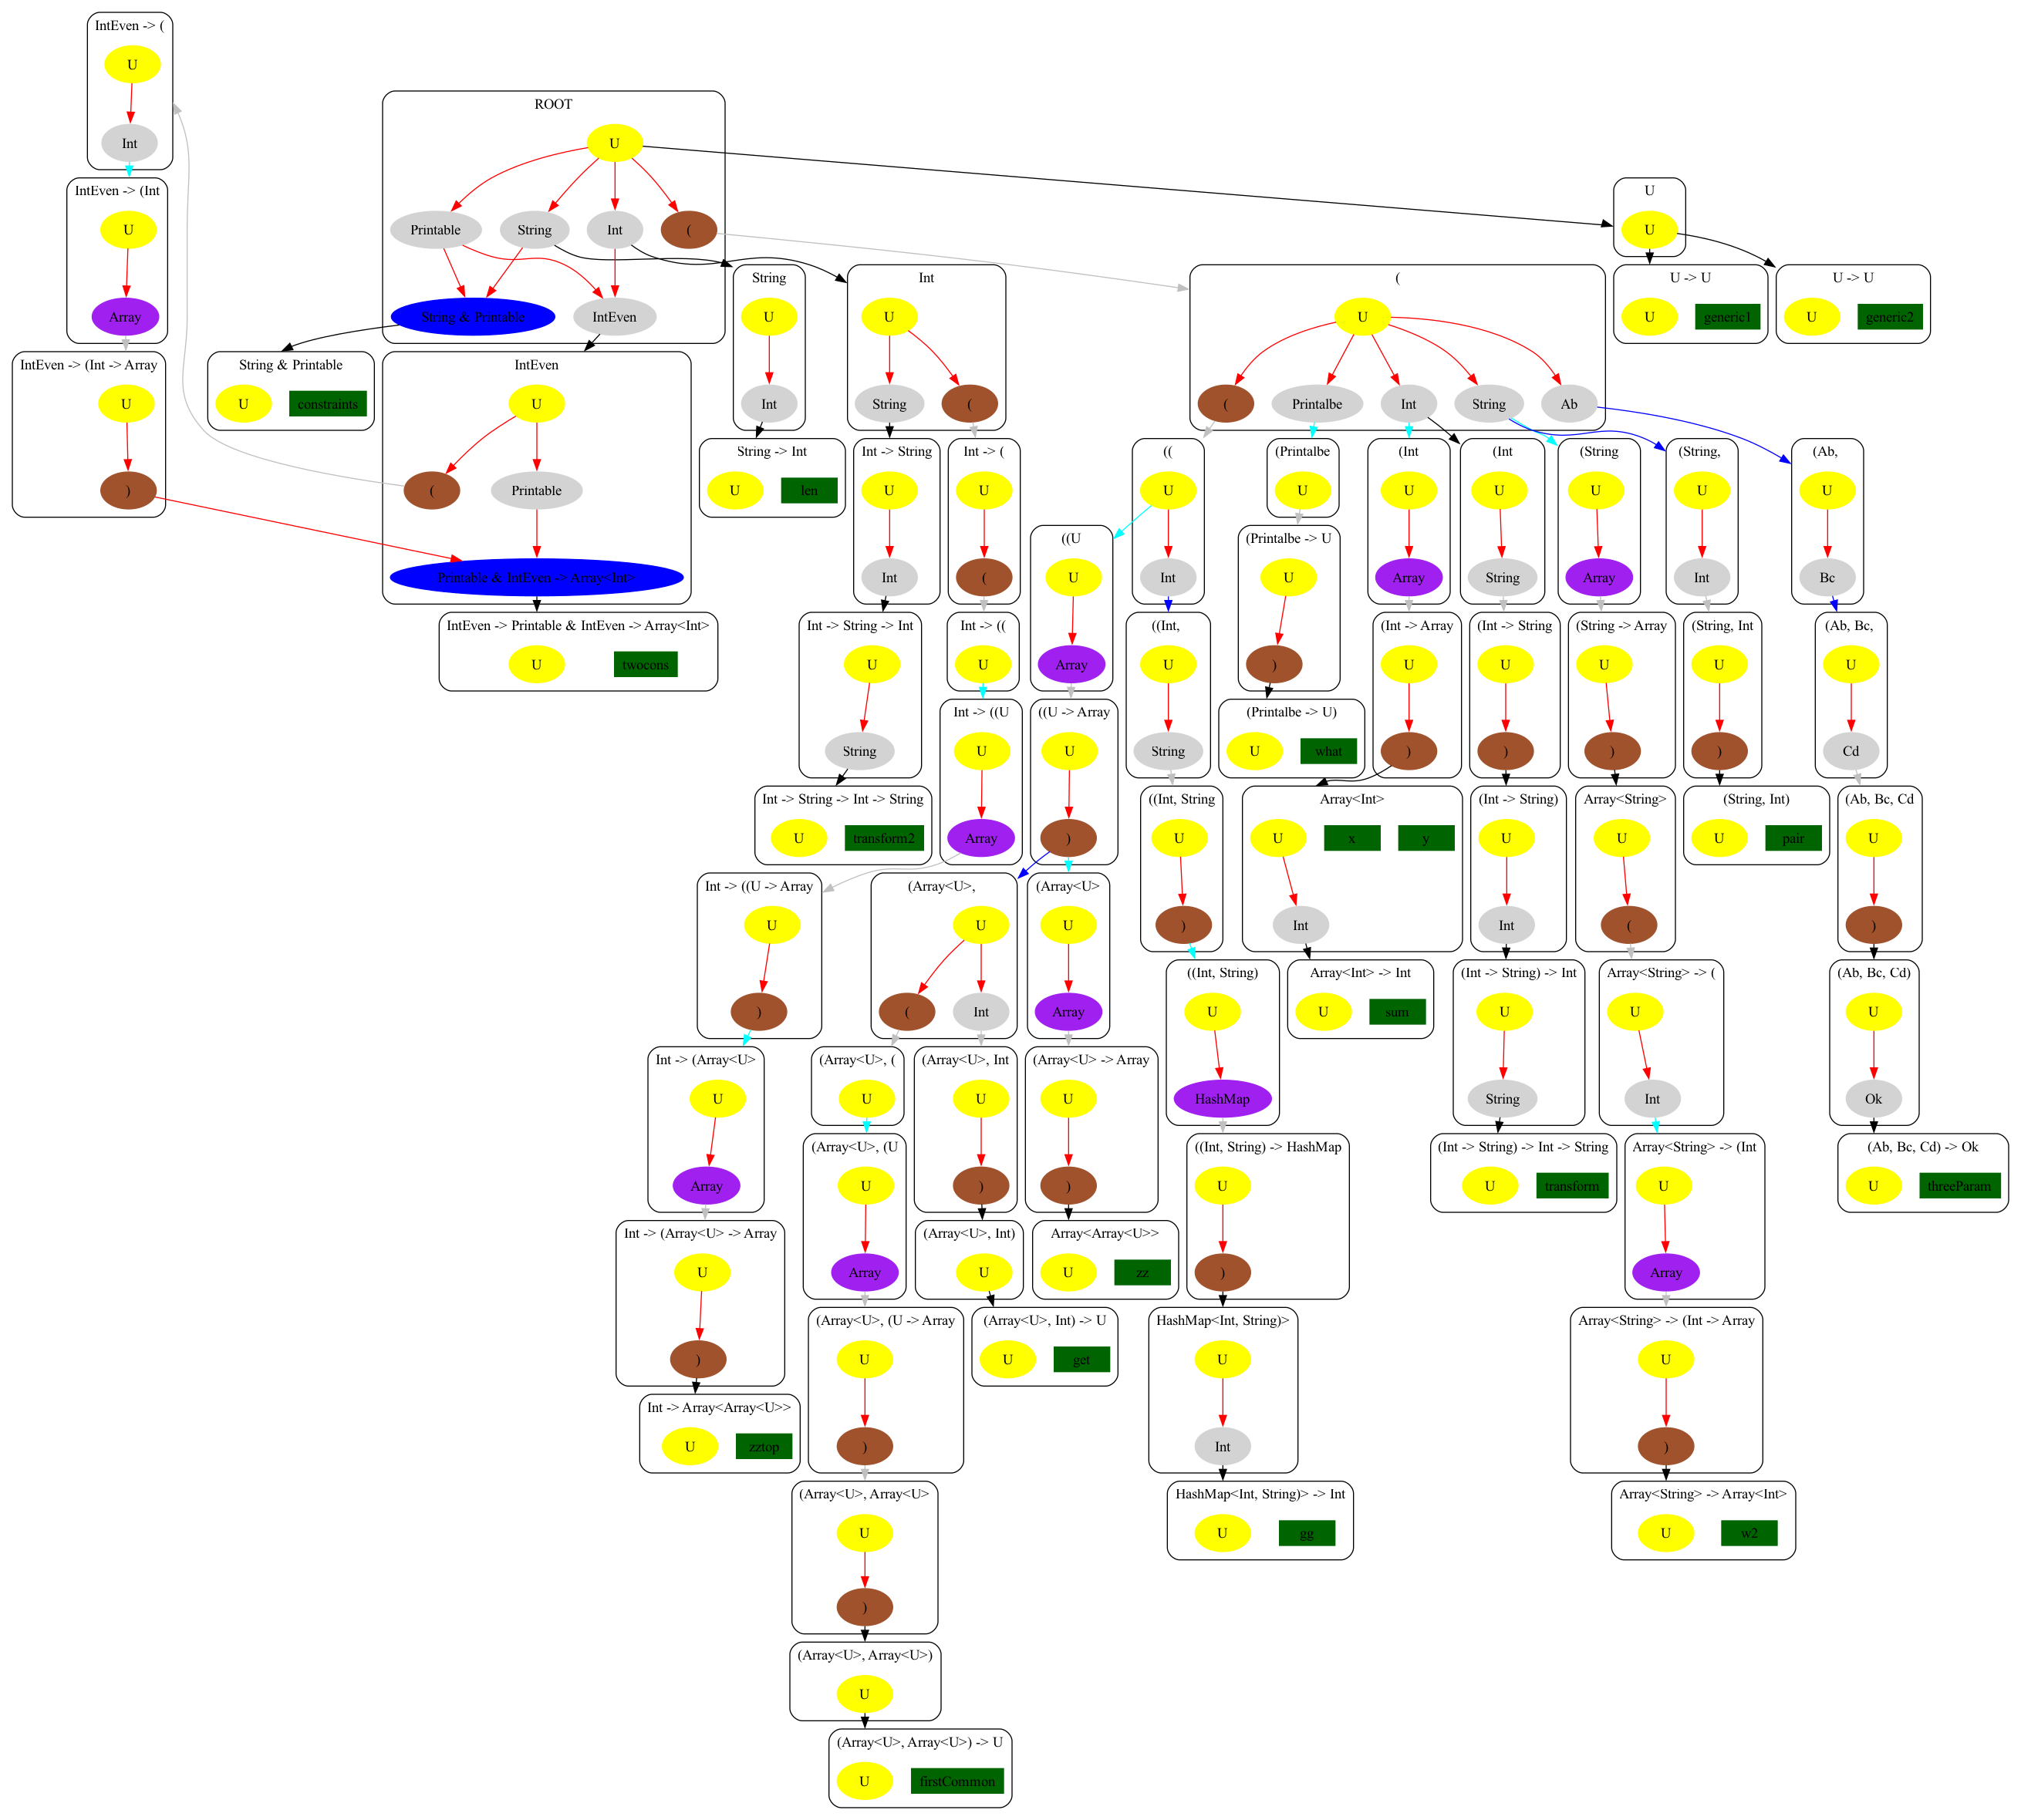
\includegraphics[width=0.8\columnwidth]{images/search_index.png}
	\end{figure}
	
	
	\begin{lstlisting}[caption={Множество деклараций на основании которых построен поисковый индекс на рисунке ~\ref{fig:1}},label={search_index_declarations}]
		len : String -> Int
		sum : Array<Int> -> Int
		transform : (Int -> String) -> Int -> String
		transform2 : Int -> String -> Int -> String
		generic1 : T -> T
		generic2 : T -> G
		constraints : T where T < Printable & String
		twocons : IntEven -> T where T < Printable & Array<Int>
		what : G<T> where T < Printalbe, G < Printable
		w2 : Array<String> -> Array<Int>
		zz : Array<Array<T>>
		zztop : Int -> Array<Array<T>>
		gg : HashMap<Int, String> -> Int
		x : Array<Int>
		y : Array<Int>
		pair : (String, Int)
		get : Int, Array<T> -> T
		firstCommon: Array<T>, Array<T> -> T
		threeParam: Ab, Bc, Cd -> Ok	
	\end{lstlisting}
	
	\hfill \break
	Стрелки между вершинами:
	\begin{enumerate}
		\item[--] Красные --- отношение подстановки
		\item[--] От TypeNode к Node:
			\begin{enumerate} 
				\item[--] Черные --- функциональные
				\item[--] Синие --- запятые кортежей
				\item[--] Сине-зеленые --- стрелки между дженериками и содержащими их номинативами
				\item[--] Серые --- от или к служебной вершине
			\end{enumerate} 
	\end{enumerate}
	
	\hfill \break
	Цвета TypeNode:
	\begin{enumerate} 
		\item[--] Жёлтый --- универсальный тип
		\item[--] Серый --- номинатив
		\item[--] Коричневые --- скобки
		\item[--] Синие --- синтетические ноды, для представления типов, которые заданы ограничениями
		\item[--] Фиолетовые --- бывшие номинативы с дженериками (Чтобы отличать Array<T> от Array)
	\end{enumerate}
		
	\hfill \break
	Поисковой индекс внешне похож на дерево, особенно, если смотреть на него как на множество Node. Эта особенность связана с тем, что изначальная его идея основана на префиксом дереве. А TypeNode'ы решают большую часть нюансов описанных ранее, которые связаны с определение подтипизации.
	
		\begin{figure}[!h]
		\caption{Граф подтипизации} \label{subtypegraph}
		\centering
		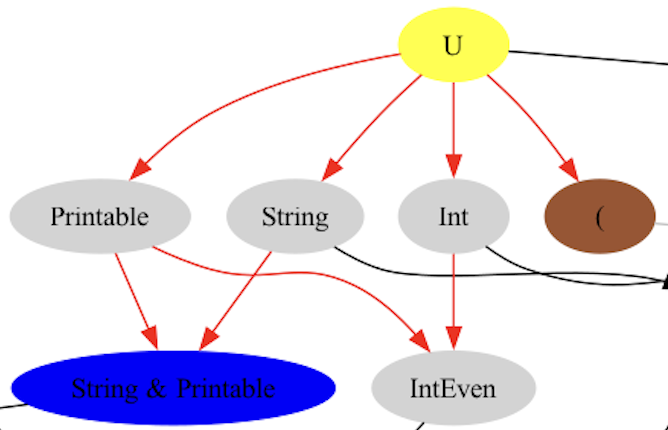
\includegraphics[width=0.8\columnwidth]{images/subtyping_graph.png}
	\end{figure}
	
	Каждая новая Node состоит из графа подтипизации, содержащей только один универсальный тип и пустого множество деклараций, которые закончились в этой ноде. При построении индекса в граф подтипизации добавляются новые типы и связи между ними.
	
	Граф подтипизации это частично упорядоченное множество построенное между типами, которые логически принажлежат одной Node, в нём также отражены и ограничения на типы. Отношения подтипизации могут связывать любые два типа. 

	\begin{lstlisting}[caption={Множество деклараций на основании которых построен поисковый индекс на рисунке ~\ref{subtypegraphhard}},label={subtyping_example}]
		T_AnBn: T where T < An & Bn
		T_AnCn: T where T < Cn & An
		T_CnDn: T where T < Cn & Dn
		AnDn : AnDn
		T_AnDn : T where T < An & Dn
		AnBnCn: AnBnCn
		T_AnBnCn: T where T < An & Bn & Cn
		T_CnT_AnDn : T where T < AnDn & Cn
		T_AnCnDn : T where T < An & Cn & Dn
	\end{lstlisting}
	
	\begin{figure}[!h]
		\caption{Более сложный пример графа подтипизации} \label{subtypegraphhard}
		\centering
		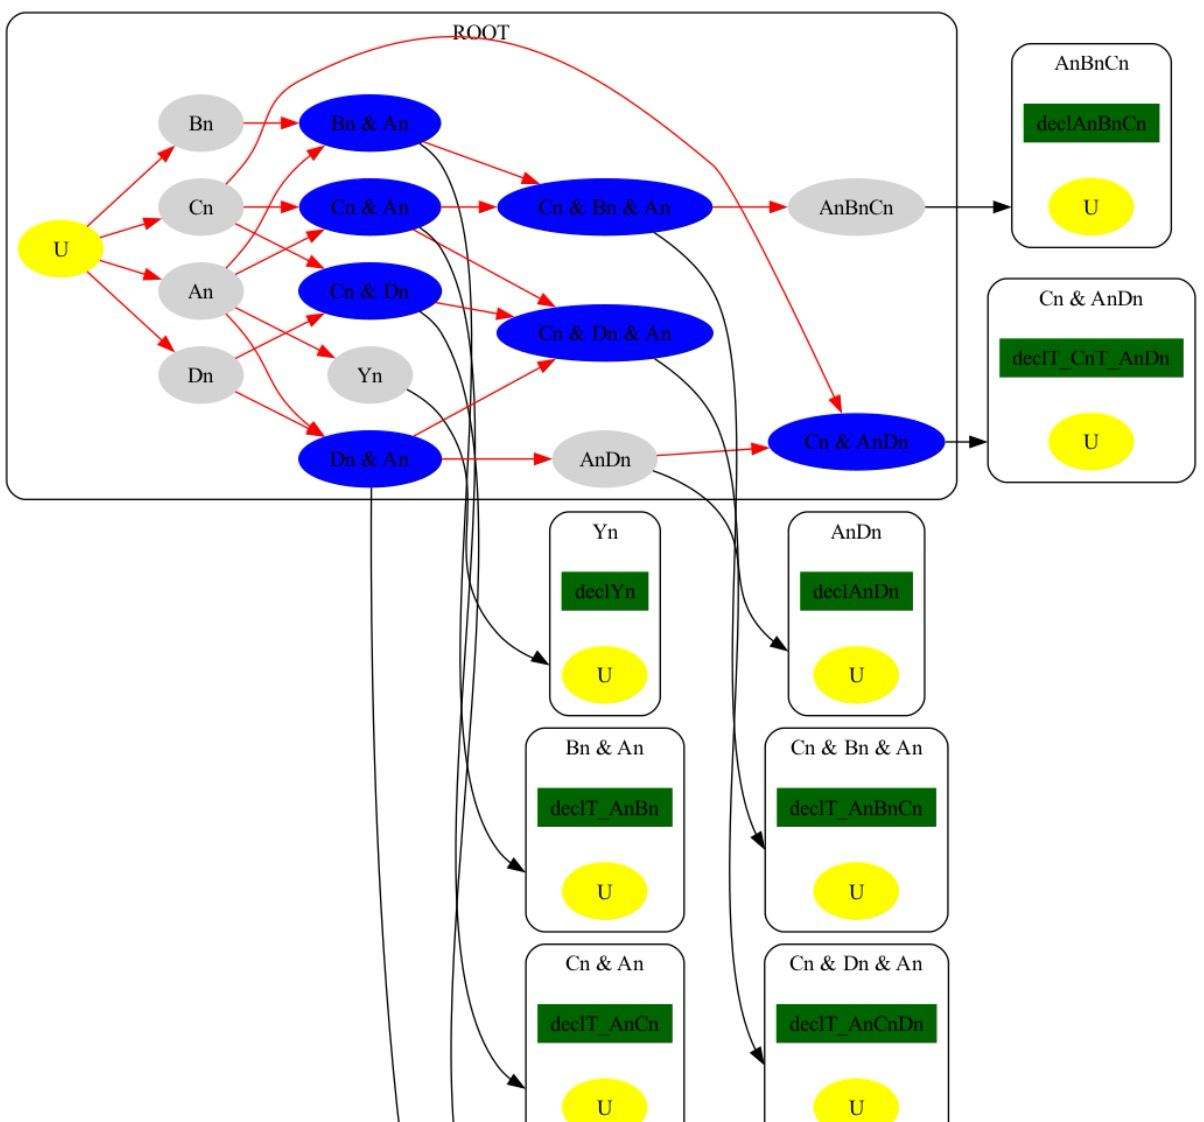
\includegraphics[width=0.8\columnwidth]{images/subtyping_hard.jpg}
	\end{figure}
	
	
	\begin{lstlisting}[caption={Отношение подтипизации для типов с рисунка ~\ref{subtypegraphhard}},label={subtyping_relations}]
        AnBnCn < An
		AnBnCn < Bn
		AnBnCn < Cn
		AnDn < An
		AnDn < Dn
		Yn < An
	\end{lstlisting}
	
	У каждой TypeNode имеется множество переходов в Node'ы, каждому переходу соответсвует пара, первым элементом которой является целевая Node, а вторая --- указатель на TypeNode, которая представляет джененрик, встречавшийся ранее и имеющий такие же ограничения или null, если эта TypeNode не является дженериком. В большем числе случаев будет иметься лишь одна пара, второе значение которой является null указателем, то есть означающим, что этот тип встречается впервые. Это верно для абсолютно всех конкрентых типов, поскольку они всегда означают одно и то же в отличие от дженериков. Для демонстрации этого --- тип \lstinline{T -> G where T < Int & G < Int} имеет два дженерика, которые, хоть и имеют общее ограничение, могут быть совершенно разными типами в отличие от типа \lstinline{Int -> Int}, где и первый и второй \lstinline{Int} указывают на одно и то же. 
	
	\begin{figure}[!h]
		\caption{Дерево построенное по декларации c типом (Int -> String) -> Int -> String} \label{subtypegraph}
		\centering
		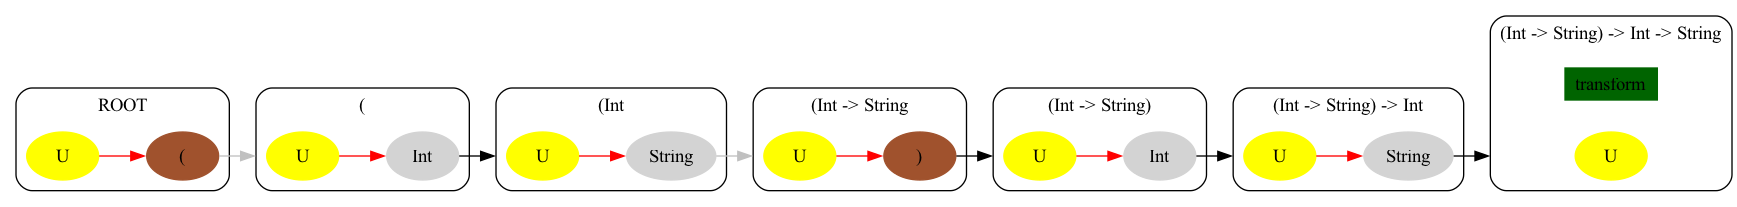
\includegraphics[width=0.8\columnwidth]{images/graph_with_hof.png}
	\end{figure}
	
	Весь индекс является «плоским». То есть функции высшего порядка хранятся и обрабатываются вне зависимости от вложенности. Функциональный тип является подтипом универасального, что так же отражено в графе подтипизации представленного TypeNode'ами. Однако важно учитывать, что и между функциональными типами могут быть подстановки, от чего сопостовлять функциональный тип целеком одной TypeNode недостаточно. Решением этого вопроса является использование двух специальных TypeNode  \lstinline{"("} и  \lstinline{")"}. Открывающаяся скобка в графе подставиммости внутри Node представлена TypeNode. Однако семантически это значит что подставима не одна ли открывающаяся скобка, а тип, который представлен между открывающей и соответствующей закрывающей скобками. Это имеет прямую аналогию с тем какой смысл скобки имеют в строках.
	
	Номнативы с дженериками в некотором роде подобны функциональным типам. Они точно так же подставляемы на позицию универсального типа, и у них точно так же могут быть отношения подтипизации, основанные на вариантности и подставимости типов аргументов. Пример, хоть может и не релевантный к большей части популярных совеременных языков --- \lstinline{Array<Int -> T> where T < Printable}, тем не менее ясно показывает что тут не обойтись одной TypeNode, в связи с тем что подставимость может зависеть от внутренностей. Решением данного вопроса является приведение дженерика к виду функционального типа. Для примера \lstinline{Array<T>} преобразуется в \lstinline{T -> Array*}. Астериск носит вспомогательный характер, означающий, что это не то же самое, что и тип, ничем не параметризованный и имеющий такое имя (\lstinline{Array}), и больше не несущий никакой смысловой нагрузки. Такой подход к трансформации джененрик параметризованных типов имеет приемущество, в первую очередь связанную с тем, что это автоматически учитывает вариантность и встраивается в текущую концепцию поискового индекса, а добавление и поиск происходит аналогично тому, как это делается для функционального типа.
	
	Поисковой индекс, организованный подобным образом, имеет приемуществом ещё и возможность распаралеливать вычисления.
	
	Важной возможностью такой структуры является способность устанавливать отношение подтипизации и для функциональных типов, которыми в частности представлены дженерики.
	
	\subsection{Добавление декларации в поисковый индекс}
	Операция добавления происходит итеративно, на каждом шаге имеется Node и тип, для которого необходимо вернуть продолжение, то есть соответсвующую TypeNode. Для разных типов этот процесс различен.
	
	Для функции создаётся служебная TypeNode, соответсвующая открывающейся скобке. По ней делается переход в следующую Node. Далее рекурсивно вставляется входной тип функции. Затем из продолжения переход в дальнейшую Node, в которую рекурсивно вставляется выходной тип функции. Далее по аналогии служебная TypeNode, соответствующая закрывающейся скобке. Стрелка-переход между входным и выходным типами является функциональной стрелкой, а стрелки после открывающейся скобки и перед закрывающейся --- служебные.
	
	Для кортежа также вставляются служебные TypeNode для скобок, между которыми вставляются типы, которые являются частями кортежа. Стрелки между ними соответсвуют запятым.
	
	Для номинатива, если он не параметризован, то просто добавляется в текущую Node. А если у него есть дженерик, то эта конструкция разварачивается в функцию, которая на входе имеет тип соответсвующий дженерику, а на выходе номинатив без параметров. Эту функция вставляется почти так же как обычная функция высшего порядка, за ислючением что между входным и выходным типом функциональная стрелка имеет особую пометку, сообщающую о том, что изначально это был параметризованный номинатив. 
	
	Подробности принципов работы лучше смотреть непосредственно в исходном коде~\cite{sourcecode}.
	
	\subsubsection{Добавление типа в граф подтипизации}
	Добавление типа в граф подставляемости отличается для конкретных типов, то есть представленных в языке, и типов синтетических, то есть таких, которые определяются ограничениями.
	
	Для конкретных типов алгоритм вставки следующий. Создаётся множество старших типов, которые будут динамически обновляться. Изначально в него добавляется универсальный тип, поскольку он является старшим к любому прочему. Затем проводиться операция «проталкивания» вниз. Для типов из множества старших перебирается множество непосредственных детей, для которых проверяется что этот ребёнок больше вставляемого типа (является предком), если это так, то он добавляется в множество страших типов. Если после проведения этой процедуры для конкретного старшего типа не один из его непосредственных детей не оказался старшим по отношению к вставляемому, то вставляемый становиться дочерним по отношение к рассматриваемому старшему. Если в таком случае вставляемый становиться старшим по отношению к какому-либо ребёнку старшего типа, то он переподвешивается как ребёнок к вставляемому. Таким образом новая TypeNode, соответсвующая вставляемому типу, становиться на своё место. Далее для прочих типов необходимо проверить не являются ли они дочерними к добавляемому. Эту процедура можно значительно ускорить заранее сообщая информацию ближайщих старших и младших типах.
	
	Для TypeNode, представляющей синтетический тип так же инициализируется множестсво старших, которые изначально добавляются заданные ограничения. Процедура вставки представляет собой нахождение нижней грани множества старших TypeNode в полной решётке~\cite{completelattice}. Если для двух TypeNode из множества существует нижняя граница, то она заменяется на эту соответсвующую TypeNode, представляющую эту границу. Если нижняя граница ещё отсутствует в ЧУМ~\cite{poset}, то она добавляется. Все эти операции, конечно же, учитывают необходимость переподвешивания вершин.
	
	Стоит отметить факт, что функциональные типы являются полноценными участниками этой схемы.
		
	Подробности того как это происходит лучше смотреть в исходном коде ~\cite{sourcecode}.
	
	\subsection{Поиск с учётом вариантности}
	Поиск с учётом вариантности напоминает поиск TypeNode по соответсвующему типу. Отличие состоит в том, что при последовательном спуске при поиске точного типа, переход делается не в одну Node, следующую из текущей TypeNode, а в несколько Node из нескольких TypeNode. Соответсвующие TypeNode берутся как старшие или младшие к TypeNode представляющей точное совпадаение, что определяется во вариантностью, принципы вычисления которой будут описаны ниже. Таким образом получается не одна подходящая TypeNode, а множество, для каждой из которых в дальнешем будет проведена процедура поиска с соответсвующей декларацией. 
	
	\subsubsection{Вычисление вариантности}
	Тип может быть ковариантным (+), контравариантным (-), инвариантным (0), бивариантным (∞), в зависимости от своего положения --- входная позиция функции, выходная позиция функции, дженерик параметр, тип в кортеже. Наиболее интутивными можно считать следующую конфигурацию --- функция контравариантна по входному типу, функция ковариатна по выходному типу, номинатив с дженериком инвариатен, кортеж ковариантен по каждому типу. Можно ещё сказать, что тип по отношению сам к себе является ковариантным. Изначально тип ковариантен, далее, если он является составным, то для его частей вычисляется перемножение вариантностей на основании конфигурации и дошедшего до данного места значения вариантности. Перемножение происходит по таблице на рисунке \ref{variancemultiplication}. 
	
	\begin{figure}[!h]
		\caption{Таблица перемножения вариантности} \label{variancemultiplication}
		\centering
		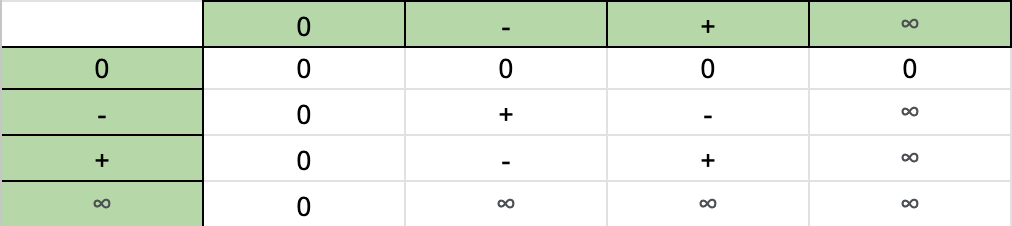
\includegraphics[width=0.8\columnwidth]{images/variancemultiplication.png}
	\end{figure}
	
	\subsection{Конструирование выражения}
	Конструирование выражений можно рассматривать как композицию функциональных типов. Выходной тип первого типа\lstinline{A -> B} должен совпадать с входным второго \lstinline{B -> C}. Проверку равенства двух типов можно осуществить одновременно совершая одинаковые шаги в двух местах. Кроме того можно совершать шаги с учётом вариантности, так чтобы выходной тип первого типа был подтипом второго. То есть алгоритм композии состоит в том чтобы сначала удовлетворить входной тип первого функционального типа, а затем начиная с этого места совершать соответсвующие шаги из корня дерева. Нюансы касающие параметров со значениями по умолчанию и другие так же естесвенно встраиваются в этот алгоритм.
	
	По другому на алгоритм можно посмотреть как на зеркальный поиск. Изначально находится множество вершин, тип пути которых соотвествует входному типу первой функции. Далее для каждой такой вершины \lstinline{A} и корня дерева делаются зекральные шаги (то есть одинаковые вплоть до совпадения дженериков), и в тех Node'ах, которые входят в путь из \lstinline{A}, где имеются декларации, эти декларации запоминаются как внутренняя часть композиции. А по зеркальным вершинам которые соответвуют путям вышедших из корня в дальнейшем делается проход соответсвующий выходному типу, и декларации которые встречаются в достигнутой вершине становятся наружней частью композии функций. Стоит обратить внимание что внутренний зеркальный проход можно делаеть не в точности, а в соответсвии с вариантностью. Итогу получается множество пар деклараций, которые в композии будут иметь заднными входной и выходной типы.
	
	\chapterconclusion
	Описанные алгоритмы позволяют структурно работать с типами, учитывая концепции систем типов, такие как вариантность, наследование, функции высшего порядка, номинативы с дженериками и прочее.
	
	\chapter{Анализ решения}
	Данная глава содержит технический обзор полученного решения и описание методологий проверки качества.
	
	\section{Обзор решения}
	Предыдущая глава содержит большую часть информации о теоретическом аспекте решения, в данной секции приводится общий обзор компонент и рассматривается ряд технических моментов.
	
	Для начала стоит подробнее рассказать о выборе инструментов, в частности языка разработки. Предпочтение было отдано языку программирования zig~\cite{zig}, который в первую очередь расчитан на разработку системного програмного обеспечения, с ручным управлением памятью. Выбор основан необходимостью написания быстрого и ресурсоёмкого приложения, что имеет две причины. Во-первых подобная утилита относиться к классу инструментов разработчика, отчего должна обеспечивать быстродействие и бережливое отношение к ресурсам хостящей машины. Во-вторых именно ручное управление памятью в совокупности со знанием алгоритмов и принципов устройства компьютеров, позволяет получать самые эффективные решения. Исходя из принципов организации структуры данных и алгоритмов можно сделать вывод, известный всем кто когда-либо писал на ассемблере, о том что основные задержки связаны именно с доступом к памяти при условии, что прочие операции выполняются за константное время. Это явление принято называть «стеной памяти» (eng: «Memory Wall»~\cite{memorywall}). Предпочтение языку zig было отдано и по некоторым другим соображениям, во-первых это механизм вычислений во время компиляции, который можно применить в качестве дальнейших оптимизаций. Это логически соответствует тому что информация о декларациях целевого языка может быть известна уже на этапе компиляции. То есть поисковой индекс можно ещё более оптимально разместить в памяти. Кроме того, zig --- открытый язык с идеологией устойчивого развития и может компилировать код под самые разные архитектуры. В любом случае, это может быть делом вкуса, но факт в том что полученное решение весьма эффективно.
	
	Проект разбит на несколько компонент: парсер, поисковой движок, визуализатор, кэш --- граф подставимости и драйвер. Все это компоненты используют структуры, которые можно разделить на два класса --- структуры описания информации о декларациях и типах: Declaration, Nominative, Function, List, Type, Constraint и структуры для описания фрагментов поискового индекса: Node, TypeNode, Following(ребро и семантическое информация о нём).
	
	\begin{figure}[!h]
		\caption{Схема перемещения данных между основными компонентами} \label{dataflow}
		\centering
		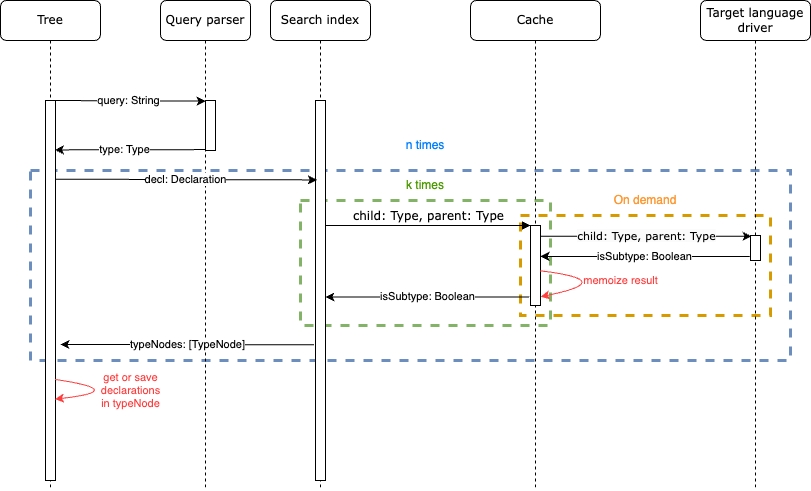
\includegraphics[width=0.8\columnwidth]{images/dataflow.png}
	\end{figure}
	
	Парсер не является критическим по производительности местом. Его реализация не соответсвует типам LL-(k) или LR. Однако он справляется с основной задачей --- разбором типовго выражения.
	
	Поисковой движок естественным образом использует поисковый индекс. Он представлен рядом методов структур Tree, Node и TypeNode. Для спуска по дереву, от его вершины к корню, то есть последовательному удовлетворению поискового запроса, в методы передаются указатели на соотвутсвующие вершины и тип, для которого необходимо совершит поиск.
	
	Визуализация поискового индекса осуществляется при помощи утилиты dot из пакета graphviz~\cite{dotgraphvizdocumentation}. По имеющейся информации о вершинах и рёбрах формируется текстовый файл, который и служит входной информацией для визуализатора.
	
	Кэш, необходимый для того чтобы сохранять информацию о подставимости типов, а не обращаться к драйверу целевого языка, представлен точно такой же структурой, что и поисковый индекс. В отличие от Node, в которой только хранятся типы, по которым можно делать дальнейший переход, в кэше постепенно накапливается информация вообще о всех типах и их отношениях подтипизации. Стоит заметить что алгоритмы проверки подтипизации в кеше несколько отличаются от проверки подтипизации при помощи кеша, во втором случае проверка что один тип явлется подтипом другого осуществляется через проверку вхождения его в множество верхних граней дочернего. А проверка при отсутствии одного из типов к кэше делается через обращение к оракулу драйвера целевого языка, то есть функции принимающей два типа о определяющей связанны ли они отношением подтипизации.
	
	Стоит пару слов сказать о возоможности распаралеливать поиск и другие операции с деревом. Это стало возможно благодоря древовидному представлению поискового индекса и итеративности алгоритма поиска. Что может иметь смысл как для возможности одновременного поиска ответов на несколько запросов в одно и то же время, так и для ускорения поиска с учётом вариантности или конструирования выражений.
	
	\section{Сравнение с существующими решениями}
	Аналоги, к которым относятся Hoogle~\cite{hoogle}, Cloogle~\cite{cloogle} и Inkuire~\cite{inkuire}, в первую очередь заточены под конкретный язык, то есть решают более специфичную задачу и, как будет показано ниже, используют более наивные подходы, а кроме того они не способны конструировать выражения, состоящие их нескольких деклараций.
	
	\subsection{Hoogle}
	Hoogle, пожалуй, самое ранее из решений, которое решает задачу поиска деклараций, как обычный поиск по имени, который выходит за рамки рассмотрения данной работы, так и поиск по типу. Отличительной особенностью является то, что в поисковую выдачу могут входить декларации, не точно соответвующие запросу. Кроме того, hoogle не имеет механизма, позволяющего учитывать наследование и ограничения в общем виде. 
	
	Поиск происходит в два этапа~\cite{hooglereview}. Сначала для заданного запроса считается «отпечаток» , в котором учитывается арность, колличество конструкторов и три самых редких имени в функции. По этому отпечатку находится 100 кандидатов, которые попадают на вторую фазу. Во второй фазе идёт отсеивание невалидных кандидатов, которое возможно благодаря тому, что можно проводить более детальное сравние на уже меньшей выборке.  Как показывает практика, выбранный подход оказался весьма успешным для haskell. Этому же способствовала система ранжирования кандидатов с весами, полученными путём голосования. К минусам можно отнести то, что это решение весьма специфичное для целевого языка и к тому же не позволяет конструировать выражения. 
	
	\subsection{Cloogle}
	Cloogle --- решение для языка Clean~\cite{clean} использует несколько другой подход. Поисковый индекс представляет из себя дерево, спуск по которому соответсвует уточнению типа. Так для родительской вершины \lstinline{a -> Int} дочерними могут быть \lstinline{Int -> Int} или \lstinline{String -> Int}. Этот достаточно интуитивный подход, но он так же не позволяет работать с множеством нюансов систем типов, такими как наследование, механизм ограничений и вариантностью (например дженериков~\cite{kotlingenericsandvariance}). 
	
	Camil Staps (автор cloogle) на вопрос о сравнении hoogle и cloogle ответил: «The algorithm is crucially different from Hoogle's, which does not rely on unification.» (перевод: Этот алгоритм существенно отличается от алгоритма hoogle, который не опирается на унификацию.) 
	
	\subsection{Inkuire}
	Наиболее близким с точки зрения определения системы типов является Inkuire, реализованный для поиска в языках Scala и Kotlin. Стоит обратить внимания на язык запросов, который может показаться излишне загруженным, для примера \lstinline{<K, V> Map<K, V>.(K) -> V?} или \lstinline{(String) -> Int} или \lstinline{Int.() -> String} или \lstinline{<T> List<T>.((T) -> Boolean) -> Pair<List<T>, List<T>>}. Подобная запись требует точного знания сигнатур деклараций, необходимости явной записи дженерик параметров и лишних скобок. Сложность формирования поискового запроса не такая маленькая проблема, как кажется на первый взгляд, потому что во-первых легче ошибиться, а во-вторых требуется гораздо больше умственных усилий для формирования запроса, например нужно явно определять является ли один из входных типов ресивером или же обычным параметром. В случае, если ресивер является номинативом с дженерик параметром, как в последнем примере, то запрос может стать излишне перегруженным.
	
	В отличие от предыдущих аналогов в Inkjure используется более гибкий подход, который позволяет учитывать особенности ООП языков, такие как наследование и вариантность. Он также использую концептуальную модель графа подстановки.
	
	К сожалению, у Inkjure нет документации или сколь угодно поверхностного обзора устройства поискового движка. Единственное, о чём авторы рассказали в видео презентации~\cite{inkuirerepresentation} --- то, что утилита способна учитывать вариантность и наследование. В Inkuire собирается база данных деклараций для которых сохраняется множество практически вся известная информация, а сам поиск происходит как-бы через запросы к этой базе данных. 
	
	\subsection{Итоги сравнения}
	Существующие аналоги используют специфичные подходы к решению задачи, в то время как предложенное в работе опирается на фундаментльные приципы систем типов и даёт более общий механизм, позволяющий учитывать вариантность, наследование, ограничения в наиболее общем виде. Кроме того, в описанное решение естественным образом встраивается концепция конструирования выражений, а визуализация показывает насколько данный подход естественен и удобен для работы с типами.
	Быстродействие поиска декларации по предложенному поисковому индексу обеспечивается не за счёт приблизительного поиска, а за счёт того, что на каждом шаге не делается лишних действий, то есть никогда не рассматирваются заранее невалидные кандидаты. 
	
	\section{Валидация решения}
	Данный раздел описывает каким образом проверяется качество работы каждого из компонентов по отдельности и всей утилиты в целом. 
	
	\subsection{Тестирование парсера запросов}
	Для тестирования парсера запросов лучше всего подходит самое обычное юнит-тестирование, то есть ряд тестов, где на вход в строковой форме задан поисковой запрос, а для разобранного результата совершаются проверки на соответсвие с ожидаемым. Код тестов представлен в query.zig. Тесты проверяют во-первых что правильно разбираются конструкции такие как --- номинативы, функциональные типы, кортежи, номинативы с дженериками, функции высшего порядка. Так же имеются тесты проверяющие что разобранные типы, имеющие одинаковые имена, совпадают вплоть до указателей на соответсвующие структуры. Например, в \lstinline{Array<T> -> Iterable<T>} первое и второе вхождение \lstinline{T} должны указывать на одну и ту же структуру, представляющую соответсвующий элемент. Кроме этого, проверяется, что правильно разбираются ограничения, указанные после ключевого слова \lstinline{where}. Тестируется, что эти ограничения присоединяются к соответсвующим типам.
	
	\subsection{Тестирование поискового индекса}
	Тестирование поискового движка, как отдельного компонента, состоит из проверок на добавление деклараций по соответствующим им типам, проверок на точный поиск, на поиск с учётом заданной вариатности, на правильное размещение вложенных типов в графе подставляемости. Тесты приведены в файлах папки src/engine/tests. Этими тестами проверяются все известные случаи и нюансы. Часть тестов нацеленны на проверку корректность построения графа подтипизации.
	
	\subsection{Тестирование визуализатора}
	Тестирование визуализатора состоит в основном из проверки корректности названий Node пути пройденному до этой вершины, и TypeNode на соответсвие типам. Также ряд тестов проверяет, что формируемый текстовый файл, который будет использован на вход утилиты dot, содержит правильную информацию.
	
	\subsection{Общие тесты}
	Кроме специфичных вышеперечисленных тестов, реализован ряд общих проверок, в которых проверяется, что в процессе работы не происходит утечек памяти, и не происходит лишних аллокаций, то есть указатели на структуру совпадают на одном и на другом концах программы.
	
	\subsection{Проверка качества утилиты в целом}\label{e2etests}
	Поскольку утилита направлена на решение весьма практичной задачи, важно проверять её работоспособность в реальных условиях. Схема проверки весьма простая и опирается на принцип --- если код компилируется, то он корректный.
	
	И так, после процедуры поиска имеется запрос (тип, кандидаты для которого ищутся) и найденные декларации. Все остальные декларации не являются подходящими под этот тип. Поэтому схема проверки следующая --- генерируем код, состоящий из  переменной с типом соотетсвующей декларации, и присваивания этой переменной в другую переменную тип которой соответсвует типу запроса. Такой код должен компилироваться для всех найденных деклараций и выдавать ошибку компиляции для прочих. Такой способ проверки может быть реализован во многих языках. Ниже приведён пример для языка kotlin. Проверка того, что кандидат подходит под запрос происходит во второй строчке функции main. Это как раз соответсвует тому, что тип декларации подставим вместо типа запроса.
	
	\begin{lstlisting}[caption={Схема валидации решения для языка kotlin},label={validation_scheme}]
		fun <T> foo(x: Boolean): List<T> = throw NotImplementedError()
		
		fun main() {
			val candidate: (Boolean) -> List<Int> = ::foo
			val query: (Boolean) -> Collection<Int> = candidate
		}
	\end{lstlisting}
	
	В листинге \ref{validation_scheme} приведён пример кода, который не скомпилируется, потому что тип \lstinline{(Boolean) -> List<Int>} нельзя использовать там, где ожидается \lstinline{(Boolean) -> Collection<Boolean>}. Компилятор напечатает ошибку вида «Type mismatch: inferred type is (Boolean) -> List<Int> but (Boolean) -> Collection<Boolean> was expected».
	
	\begin{lstlisting}[caption={Пример кода, который не скомпилируется},label={validation_scheme}]
		fun <T> foo(x: Boolean): List<T> = throw NotImplementedError()
		
		fun main() {
			val candidate: (Boolean) -> List<Int> = ::foo
			val query: (Boolean) -> Collection<Boolean> = candidate
		}
	\end{lstlisting}
	
	Надёжность данного способа валидации решения упирается только в правильность работы компилятора. Хотя сама схема проверки и кажется сложной с вычислительной точки зрения, поскольку для каждого поискового запроса нужно совершить столько компиляций, сколько всего есть деклараций, её, однако, можно ускорить, если добавить предварительную проверку арности типов и другие проверки, которые исключат заранее невалидных кандидатов.
	
	Идеальным результатом может считаться, если все ожидаемо компилирующиеся программы скомпилируются, а прочие нет. Однако, допустимо, что могут возникнуть крайние случаи, которые не будут корректными. Поэтому можно замерить процент корректных запусков компилятора, где результат совпадает с ожидаемым ко всему колличеству запусков. Это назовём процентным показателелем качества. Также можно систематизировать случаи корректной и некорректной работы утилиты и проанализировать полученные результаты.
	
	Качественная реализация драйвера написанна только для непубличного языка. Утилита не покрывает лишь часть случаев, которые однако нельзя подробнее описать. Пример демострации возможностей привдён в исходном коде на примере искусственной системы типов, которая однако является весьма приближенной к настоящей. Наиболее долгой операцией является построение поискового индекса, скорость поиска и конструирования выражаения в общем случае зависят от колличества деклараций в индексе и особенностей подтипизации, однако для примеров на которых производилось тестирование в процессе написания, операции поиска и конструирования выражения выполнялись быстрее 1 миллисекунды. По памяти тестовый пример вмещается в 1 мб. В целом данную утилиту можно применять и в реальной жизни, это однако требует ряда настроек специфичных для ситуации.
	
	\subsection{Сравнение с конкурентами}
	Из описанных аналогов наиболее подходящим для сравнения является Inkuire. Основная причина в том, что он учитывает отношения подтипизации и вариантность. Количественное сравнение проводилось по 2-м критериям: средней скорости ответа на запрос и процентному показателю качества на выборке из 100 случайных типов. Результаты приведены в папке comparision исходного кода.
	
	Затрудняющим для сравнения принципов устройства является использование весьма разных языков реализации. Inkuire написанный на высокоуровневом языке scala, поддерживающим весьма много абстракций, в то время, как предложенное решение написанно на языке zig, изначально заточенным под системную разработку. 
	
	Хотя оба решения учитывают подтипизацию, способы их представления несколько отличаются. В предложенном решении для каждой отдельной Node существует свой граф подставимости, что позволяет значительно быстрее делать поиск с учётом вариантности и наследования. Кроме того, идея префиксного дерева, которое позволяет получать наглядную визуализацию деклараций в пространстве типов, является уникальной в предложенном решении. Inkuire не позволяет комбинировать отдельные декларации в выражения, в то время как это естественным образом возможно в текущем решенении. Следующее отличие в способе введения дженериков. В Inkuire это делается явно, а не на основании правила о том, что джененрик это одиночная заглавная буква. Ещё одним отличием Inkuire является выделение ресивера, что с одной стороны усложняет синтаксис запросов, но с другой даёт дополнительную точность, польза которой несколько неоднозначна, поскольку для нахождения желаемой декларации будет необходимо воспользоваться поиском два раза, в то время как в предложенном решении полноценная поисковая выдача будет получена по одному запросу.
	
	\chapterconclusion
	Решение состоит из отдельных весьма естественных компонент. Если рассматривать язык как первостепенное средство разработки, то выбор zig имел как плюсы, так и минусы. С одной стороны это весьма высокая сложность разработки, но с другой производительность и эффективность решения в совокупности с хорошим заделом для будущих улучшений.
	
	В рамках работы удолось провести лишь ограниченный анализ полученного решения. Тесты показывают концептуальную корректность и работоспособность утилиты. Однако, кроме как на непубличном языке, полноценная работоспособность не была проверенна. Это может быть исправлено в дальнейшем.
	
	%% Макрос для заключения. Совместим со старым стилевиком.
	\startconclusionpage
	Полученное решение представляет интерес, как удачный способ рассмотрения деклараций в пространстве типов. К положительным особенностям решения относятся быстрота поиска, возможность дальнейшего распаралеливания и достаточная общность решения, требующая реализации лишь одной функции для целевого языка. К минусам можно отнести возможность неучитывания некоторых специфичных особенностей системы типов целевого языка.
	
	Полученное решение способно работать с системами типов которые имеют: номинативы, наследование, номинативы с параметризацией, механизм ограничений, функциональные типы и вариантность. Драйвер целевого языка в минимальном случае должен предоставлять декларации с типами в грамматике описанной в работе, а так же уметь отвечать на вопросы подтипизации двух типов. По хорошему не хватает анализа решения с разными языками, но это весьма объёмная работа может быть выполненна в дальнешем.

	
	\printmainbibliography
	
\end{document}
